\section*{Dati e risultati}

\begin{SCfigure}[0.55][t]
    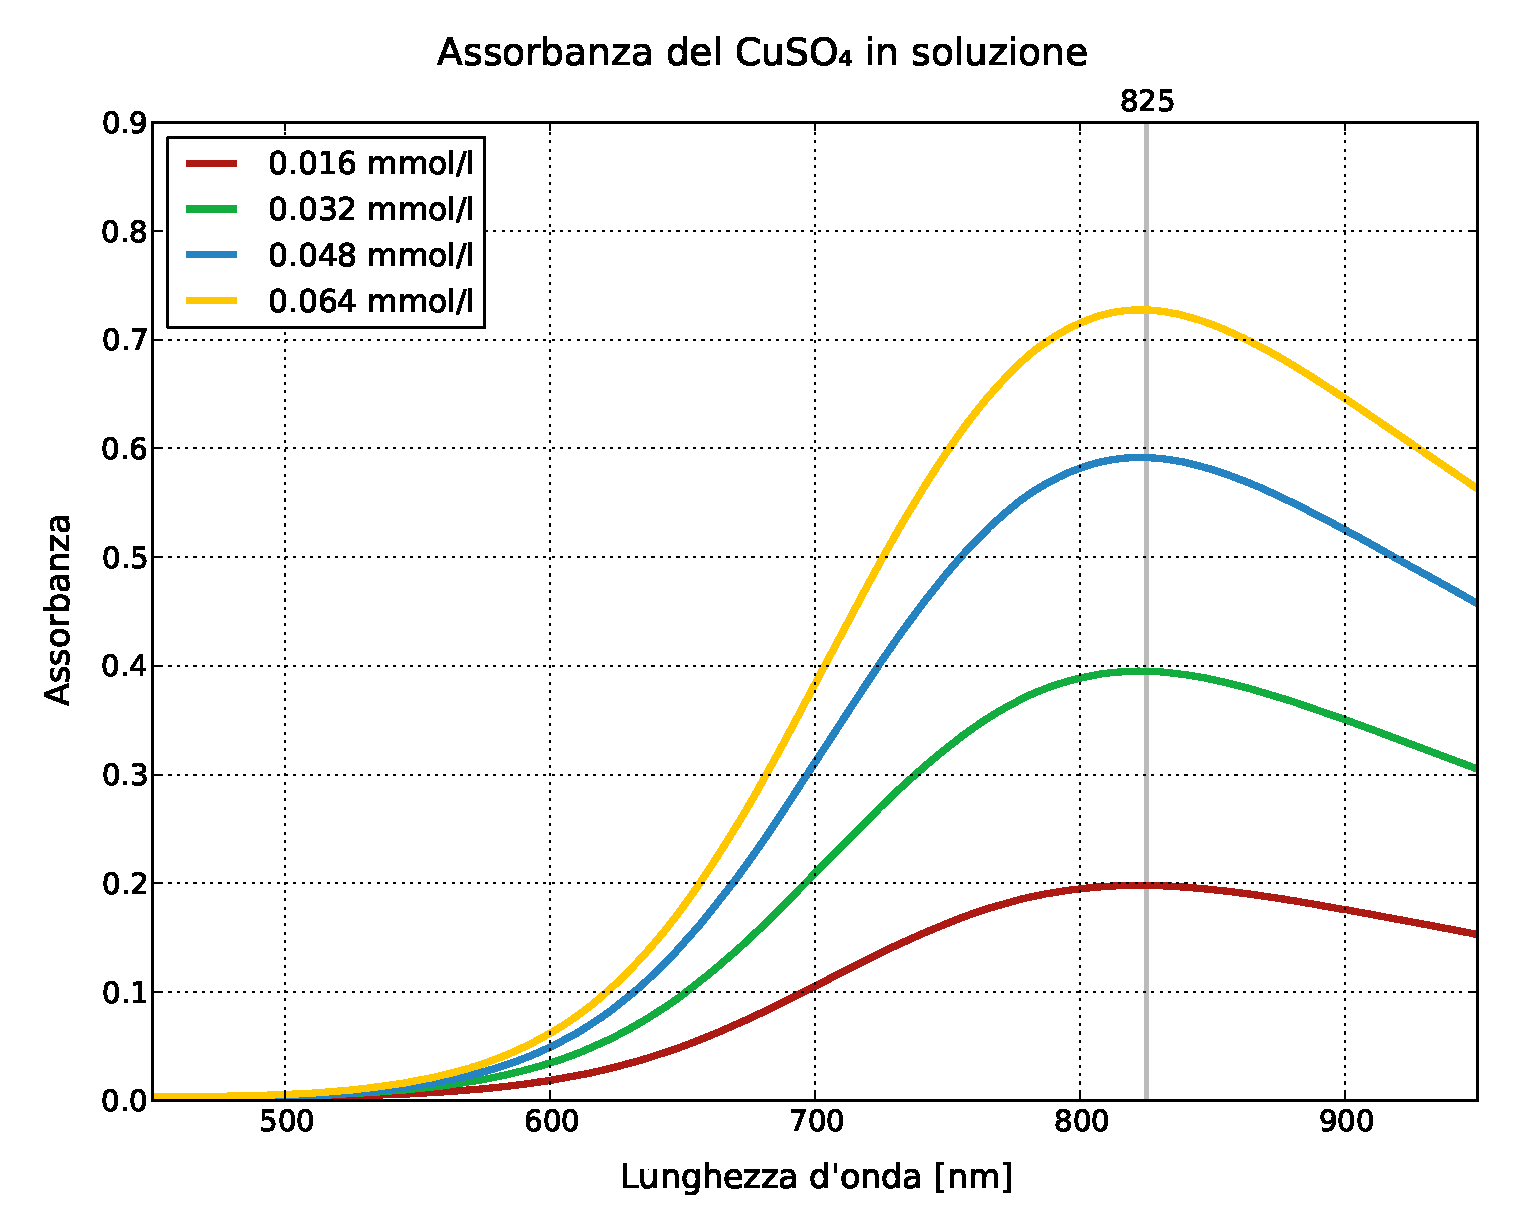
\includegraphics[scale=0.52]{concentrazioni.pdf}
    \caption{Nel grafico sono rappresentate le curve di assorbimento in funzione della lunghezza d'onda delle quattro soluzioni note.
        \`E stata inoltre evidenziata tramite una linea verticale la lunghezza d'onda di massima assorbanza $\lambda\ped{max} = \SI{825}{\nano\meter}$.
        Queste curve sono interessanti poichè spiegano il colore azzurro intenso di una soluzione di \ce{CuSO4}. Il massimo di assorbimento
        nel visibile è ad alte lunghezze d'onda, ovvero nel rosso e nell'infrarosso; la luce di colore blu invece, passa indisturbata, per cui la soluzione appare di
        colore blu. La barra colorata in basso indica approssimativamente i colori corrispondenti alle lunghezze d'onda del grafico soprastante.}
    \label{fig:conc}
\end{SCfigure}

Dal grafico in Figura \ref{fig:conc} si può osservare che l'assorbanza delle soluzioni con molarità più bassa
è stata predetta con precisione: infatti le soluzioni titolate $\SI{0.016}{\mole\per\litre}$, $\SI{0.032}{\mole\per\litre}$
e $\SI{0.048}{\mole\per\litre}$ hanno assorbanza massima a $\lambda\ped{max}$ relativamente di $0.2$, $0.4$ e $0.6$.
La soluzione titolata $\SI{0.064}{\mole\per\litre}$ invece è risultata avere assorbanza massima, sempre in $\lambda\ped{max}$,
di $0.73$. Un valore particolarmente distante dal preventivato $0.8$, ma comunque all'interno dell'intervallo di validita della Lambert-Beer.

Le curve di assorbimento mostrate in Figura \ref{fig:conc} sono interessanti poichè offrono una precisa visione d'insieme dell'assorbimento
della soluzione, sia al variare della lunghezza d'onda che della concentrazione. Inoltre si comprende come mai una soluzione di
solfato di rame sia azzurra: la luce rossa è assorbita, mentre quella blu attraversa la soluzione indisturbata.

Inoltre si può osservare che l'assorbanza è all'incirca lineare con la concentrazione. Questo fatto è mostrato meglio nella Figura \ref{fig:a_vs_c},
dove sono mostrati i valori di assorbanza in funzione della concentrazione per la lunghezza d'onda di picco $\lambda\ped{max}$.

Abbiamo eseguito una regressione lineare utilizzando solo le incertezze sulla concentrazione derivate dalle incertezze sul volume.
Le incertezze sull'assorbanza sono state considerate trascurabili in tutti i calcoli e quindi anche nella regressione, questo perché non
siamo a conoscenza dell'incertezza nelle misure del fotospettrometro.
Il coefficiente angolare della retta ricavata, riportata in Figura \ref{fig:a_vs_c},
non è altro che $\alpha$:

\begin{equation}
    \alpha = 11.6 \pm 0.4 ~ \text{l/mol}
\end{equation}

Per assicurarci che la retta di fit fosse corretta abbiamo eseguito il test del chi quadro sulla regressione. Poichè la retta deve necessariamente
passare per l'origine (quando la soluzione ha concentrazione zero, ovvero è acqua, deve avere assorbanza zero, perché l'assorbanza è misurata in
relazione a quella dell'acqua. Si veda la (\ref{eq:ass})), abbiamo 4 - 1 = 3 gradi di libertà, che è anche il valore atteso del $\chi^2$.
È risultato $\chi^2 = 10$, non compatibile con il valore teorico all'interno dell'intervallo di confidenza del 90\% da noi scelto.
Quindi abbiamo dovuto correggere le incertezze. Questo è accaduto poichè abbiamo trascurato
le incertezze sull'assorbanza. La correzione è quindi servita per calcolare le incertezze incognite sull'assorbanza, che sono risultate essere 0.01, 0.02,
0.03, 0.04 rispettivamente per le quattro soluzioni (si veda il grafico).

Ora, avendo misurato l'assorbanza della soluzione a concentrazione incognita a 825 nm, che vale $A\ped{inc} = 0.599$, siamo in grado, rovesciando la
(\ref{eq:lambeer}), di ottenere la concentrazione.

\begin{equation}
    c = \frac{A\ped{inc}}{\alpha} = 0.052 \pm 0.002 ~ \text{M}
\end{equation}

\begin{SCfigure}[0.55][t]
    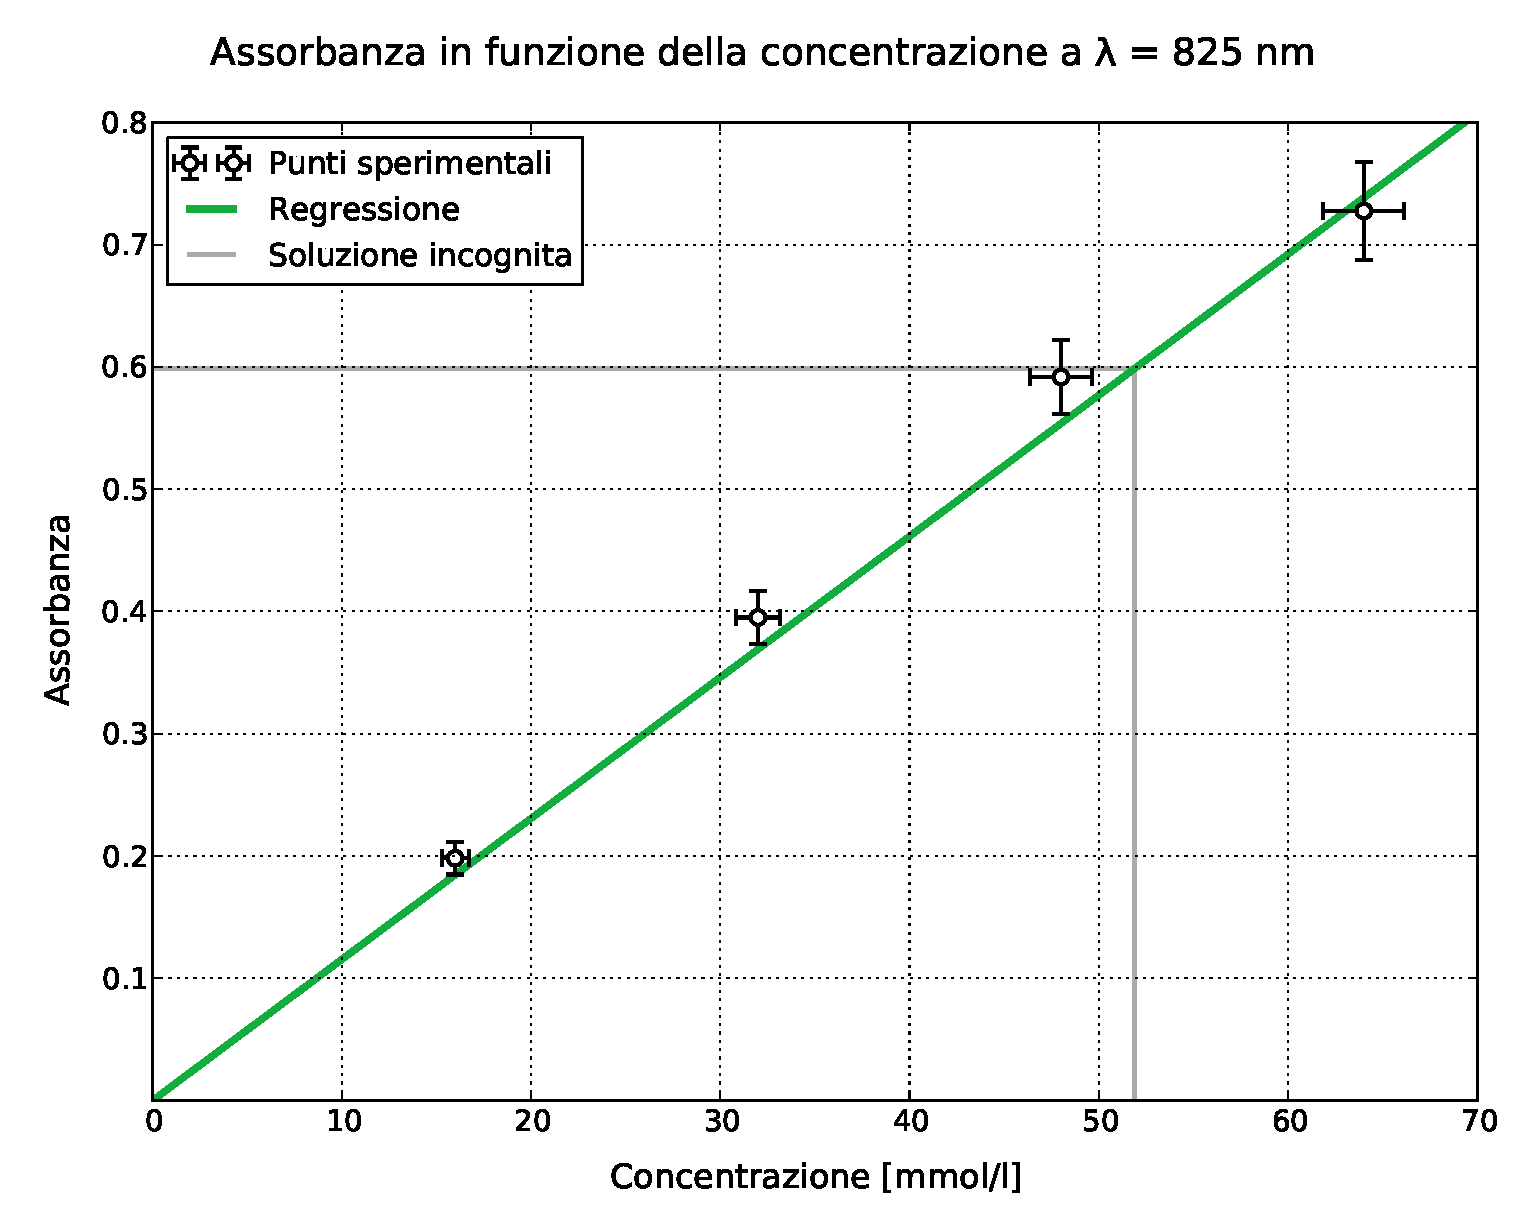
\includegraphics[scale=0.55]{retta.pdf}
    \caption{Il grafico in figura mostra l'assorbanza a $\lambda\ped{max} = \SI{825}{nm}$ in funzione della concentrazione
        per le quattro soluzioni preparate. Sono riportati sia gli errori sulla concentrazione, che le incertezze sull'assorbanza
        stimate dalla correzione delle incertezze. La retta di fit in verde 
        indica l'andamento previsto dalla legge di Lambert-Beer e ci permette di calcolare $\alpha$. In grigio è riportato
        il valore di assorbanza della soluzione incognita, dall'intersezione con la retta di fit possiamo dire che la concentrazione
        di tale soluzione è di circa 0.05 M.}
    \label{fig:a_vs_c}
\end{SCfigure}
